\documentclass[11pt]{article}
\usepackage[margin=2cm]{geometry}
\usepackage[utf8]{inputenc}
\usepackage[T1]{fontenc}
\usepackage{tikz}
\usepackage{tabularx}
\usepackage{booktabs}
\usepackage{longtable}
\usepackage{array}
\usepackage{xcolor}
\usepackage{hyperref}
\usepackage{graphicx}
\usepackage{enumitem}
\usepackage{amsmath}
\usepackage{multicol}
\usepackage{colortbl}

% TikZ libraries
\usetikzlibrary{positioning,arrows.meta,shapes.geometric,calc,decorations.pathmorphing}

% Custom colors
\definecolor{primarycolor}{RGB}{204, 102, 0}
\definecolor{secondarycolor}{RGB}{51, 102, 153}
\definecolor{accentcolor}{RGB}{0, 128, 0}
\definecolor{warningcolor}{RGB}{204, 0, 0}
\definecolor{lightgray}{RGB}{240, 240, 240}

% Hyperref setup
\hypersetup{
    colorlinks=true,
    linkcolor=secondarycolor,
    urlcolor=primarycolor,
    pdftitle={Namibia Christmas Trip 2025-2026},
    pdfauthor={Edouard Verstraete}
}

% Custom commands
\newcommand{\location}[1]{\textcolor{primarycolor}{\textbf{#1}}}
\newcommand{\booked}{\textcolor{accentcolor}{$\checkmark$ Booked}}
\newcommand{\option}{\textcolor{secondarycolor}{$\circ$ Option}}
\newcommand{\unavailable}{\textcolor{warningcolor}{$\times$ Unavailable}}
\newcommand{\tbdstatus}{\textcolor{gray}{$\bullet$ TBD}}

% Column types
\newcolumntype{L}[1]{>{\raggedright\arraybackslash}p{#1}}
\newcolumntype{C}[1]{>{\centering\arraybackslash}p{#1}}
\newcolumntype{R}[1]{>{\raggedleft\arraybackslash}p{#1}}

\title{\Huge\textbf{Namibia Family Safari}\\[0.5em]\Large Christmas 2025--2026}
\author{Edouard Verstraete}
\date{December 23, 2025 -- January 6, 2026}

\begin{document}
\maketitle
\thispagestyle{empty}

\vspace{2em}
\begin{center}
\fbox{\begin{minipage}{0.9\textwidth}
\section*{Trip Overview}
\begin{itemize}[leftmargin=*]
    \item \textbf{Duration:} 13 nights, 15 days
    \item \textbf{Travelers:} 5 persons (Edouard, brother, sister, parents)
    \item \textbf{Budget Target:} €7,000 per person (€35,000 total)
    \item \textbf{Transport:} Self-drive 4x4 (Toyota Hilux Double Cab)
    \item \textbf{Total Distance:} Approximately 2,200 km
    \item \textbf{Season:} Summer (Green Season) -- expect heat, thunderstorms, lush landscapes
\end{itemize}
\end{minipage}}
\end{center}

\clearpage
\tableofcontents
\clearpage

% =============================================================================
\section{Quick Reference}
% =============================================================================

\subsection{Budget Summary}

\begin{tabular}{@{}lrr@{}}
\toprule
\textbf{Category} & \textbf{Per Person} & \textbf{Total (5 persons)} \\
\midrule
Accommodation (13 nights) & €7,638 & €38,188 \\
Vehicle \& Transport & €725 & €3,627 \\
Activities & €651 & €3,255 \\
Park Fees & €60 & €300 \\
Meals (est.) & €200 & €1,000 \\
\midrule
\textbf{Total (excl. flights)} & \textbf{€9,274} & \textbf{€46,370} \\
\textbf{Budget Option (Mushara)} & \textbf{€7,714} & \textbf{€38,570} \\
\bottomrule
\end{tabular}

\vspace{1em}
\textit{Note: Budget option uses Mushara Lodge for Etosha (saves €1,500 pp). Kulala Desert Lodge is all-inclusive.}

\subsection{Key Dates \& Milestones}

\begin{itemize}
    \item \textbf{Dec 23 (evening):} Depart Brussels
    \item \textbf{Dec 24 (afternoon):} Arrive Windhoek, collect vehicle, drive to Sossusvlei
    \item \textbf{Dec 24--26:} Sossusvlei \& Namib Desert (3 nights)
    \item \textbf{Dec 26:} Hot air balloon flight (BOOK IMMEDIATELY)
    \item \textbf{Dec 27--28:} Swakopmund \& Skeleton Coast (2 nights)
    \item \textbf{Dec 29--31:} Damaraland (3 nights)
    \item \textbf{Jan 1--4:} Etosha National Park (4 nights)
    \item \textbf{Jan 5:} Return to Windhoek, sleep at Airport Lodge
    \item \textbf{Jan 6 (afternoon):} Departure flight to Brussels
    \item \textbf{Jan 7 (morning):} Arrive Brussels
\end{itemize}

\clearpage
% =============================================================================
\section{Route Overview}
% =============================================================================

\subsection{Complete Journey Map}

\begin{center}
\Large\textbf{\href{images/route_map.html}{→ View Interactive Map ←}}
\end{center}

\vspace{1em}
\noindent\textit{The interactive map shows all locations with markers and the complete route across Namibia. Click the link above to explore.}

\subsection{Driving Summary}

\begin{longtable}{lccll}
\toprule
\textbf{Route} & \textbf{Distance} & \textbf{Duration} & \textbf{Road Type} & \textbf{Fuel Stops} \\
\midrule
\endfirsthead
\toprule
\textbf{Route} & \textbf{Distance} & \textbf{Duration} & \textbf{Road Type} & \textbf{Fuel Stops} \\
\midrule
\endhead
Windhoek → Sossusvlei & 350 km & 5 hours & 85\% gravel & Solitaire \\
Sossusvlei → Swakopmund & 350 km & 4.5 hours & 90\% gravel & Solitaire, Walvis Bay \\
Swakopmund → Damaraland & 420 km & 5--6 hours & Mixed & Uis, Khorixas \\
Damaraland → Etosha (West) & 250 km & 4 hours & Gravel & Outjo (CRITICAL) \\
Etosha West → East (internal) & 200 km & 4--5 hours & Park roads & N/A \\
Etosha → Windhoek & 430 km & 5--5.5 hours & 95\% tarred & Otjiwarongo \\
\midrule
\textbf{TOTAL} & \textbf{2,200 km} & \textbf{27--30 hrs} & & \\
\bottomrule
\end{longtable}

\clearpage
% =============================================================================
\section{Day-by-Day Itinerary}
% =============================================================================

% -----------------------------------------------------------------------------
\subsection{Day 1: December 23--24 -- Travel \& Arrival}
% -----------------------------------------------------------------------------

\subsubsection{Timeline}

\begin{tabular}{llr}
\toprule
\textbf{Time} & \textbf{Activity} & \textbf{Cost} \\
\midrule
21:30 (Dec 23) & Depart Brussels (BRU) -- Ethiopian Airlines ET751 & -- \\
06:45 (Dec 24) & Arrive Addis Ababa (ADD) -- 1h50 layover & -- \\
08:35 & Depart ADD -- Ethiopian Airlines ET835 & -- \\
13:20 & \textbf{Arrive Windhoek Hosea Kutako Airport (WDH)} & -- \\
14:00--15:00 & Collect rental vehicle (Toyota Hilux 4x4), vehicle orientation & -- \\
15:00 & Depart for Sossusvlei (350 km, 5 hours) & -- \\
18:00 & Stop at Solitaire for fuel (82 km from Sossusvlei) & €20 \\
20:00 & Arrive at Sossusvlei lodge, check-in, dinner & -- \\
\bottomrule
\end{tabular}

\subsubsection{Notes \& Preparation}

\begin{itemize}
    \item \textbf{Change from original plan:} Drive directly to Sossusvlei instead of staying at Airport Lodge
    \item Arrive at lodge after dark -- ensure GPS is working
    \item Most of drive is gravel road -- take it slow (60 km/h), arrive safely
    \item Confirm vehicle rental pickup time and insurance (Option 3 or 4 with tire/windscreen)
    \item Check vehicle has: GPS with Tracks4Africa, dual spare tires, compressor
    \item Pick up snacks/water at airport if needed
\end{itemize}

\subsubsection{Daily Budget}

\begin{tabular}{@{}lr@{}}
\toprule
\textbf{Item} & \textbf{Cost (per person)} \\
\midrule
Accommodation (Sossusvlei, night 1) & €233 \\
Vehicle rental (half day) & €40 \\
Fuel & €20 \\
Meals & €20 \\
\midrule
\textbf{Total Day 1} & \textbf{€313} \\
\bottomrule
\end{tabular}

\clearpage
% -----------------------------------------------------------------------------
\subsection{Day 2--3: December 25--26 -- Sossusvlei \& Namib Desert}
% -----------------------------------------------------------------------------

\subsubsection{Day 2 (Dec 25): Christmas Day -- Sossusvlei Sunrise}

\begin{tabular}{llr}
\toprule
\textbf{Time} & \textbf{Activity} & \textbf{Cost} \\
\midrule
05:00 & Pre-dawn departure through private gate & Incl. \\
06:00--09:00 & Sunrise at Deadvlei, climb Big Daddy dune & Incl. \\
& Breakfast picnic at dune base & \\
10:30 & Return to lodge before extreme heat (38--40°C) & -- \\
Midday & Pool, reading, rest & -- \\
16:00 & E-bike or quad bike exploration & Incl. \\
19:00 & Special Christmas dinner at lodge & Incl. \\
\bottomrule
\end{tabular}

\subsubsection{Day 3 (Dec 26): Hot Air Balloon \& Exploration}

\begin{tabular}{llr}
\toprule
\textbf{Time} & \textbf{Activity} & \textbf{Cost} \\
\midrule
05:00 & \textbf{HOT AIR BALLOON FLIGHT} (Namib Sky) & €496 \\
& 1-hour sunrise flight over dunes & \\
& Champagne breakfast in desert & \\
& Flight certificate, park fees included & \\
10:00 & Return to lodge & -- \\
Midday & Pool and rest & -- \\
16:00 & Guided nature walk (desert ecology) & Incl. \\
Evening & Final stargazing session & Incl. \\
\bottomrule
\end{tabular}

\textcolor{accentcolor}{\textbf{BOOKED:}} Namib Sky Balloon Safaris, Dec 26, 2025 at 05:00. Booking ID: 2201704. Cost: N\$49,600 (€2,480 total / €496 per person). \textcolor{warningcolor}{\textbf{Payment required within 12 hours or booking becomes invalid.}} Conditional on securing accommodation with private gate access and flight confirmation.

\clearpage
\subsubsection{Accommodation Options: Sossusvlei (3 nights)}

\textbf{Status:} \option

\textbf{Ranked by Priority:}

\begin{enumerate}
    \item \textbf{Wilderness Kulala Desert Lodge} -- \textit{TRAVEL AGENT PROPOSAL (LEADING OPTION)}
    \begin{itemize}
        \item \textbf{Key Feature:} Private entrance to Namib Naukluft National Park
        \item Closest lodge to Sossusvlei -- first at Deadvlei at sunrise, 45 min before other tourists
        \item 23 chalets (3 chalets for 5 people)
        \item Platform design for airflow, comfortable accommodation
        \item \textbf{All-inclusive:} All meals, selected beverages (house wine, local spirits, beer, soft drinks), scheduled shared safari activities, daily laundry service
        \item \textbf{Excluded:} Premium imported beverages and champagne
        \item Activities included: dune excursions, e-bikes, quad bikes, nature walks
        \item \textbf{Cost:} \textcolor{accentcolor}{\textbf{€1,763 per person (€8,813 total for 3 nights)}}
        \item \textbf{Itinerary:} \url{https://itrvl.com/client/itineraries/691722933f2baa005c9f5709?token=Vdkl3mHfvAh1AaB62T5nssbrU8JESZajI2PyluzI7wbCHlobqrRpFEJewAFWv1BB}
        \item \textbf{Pros:} Private gate access to dunes is PRICELESS, excellent value, better availability, all-inclusive
        \item \textbf{Cons:} Less luxurious than sister property Little Kulala
    \end{itemize}

    \item \textbf{\&Beyond Sossusvlei Desert Lodge}
    \begin{itemize}
        \item 10 villas in NamibRand Nature Reserve
        \item World-class astronomical observatory with resident astronomer
        \item Location: 60 min from park entrance (compromise)
        \item Arguably Namibia's finest lodge
        \item \textbf{Cost:} €10,000--11,000 for 3 nights (5 people)
        \item \textbf{Pros:} Ultimate luxury, unique observatory experience
        \item \textbf{Cons:} No private gate access, very expensive, distance to dunes
    \end{itemize}

    \item \textbf{Sossusvlei Lodge} (Budget option)
    \begin{itemize}
        \item At Sesriem Gate entrance
        \item Convenient location, functional accommodation
        \item No private gate access (standard park entry)
        \item \textbf{Cost:} €1,500--2,000 for 3 nights (5 people)
        \item \textbf{Pros:} Good value, convenient, adequate facilities
        \item \textbf{Cons:} Not luxury, no private access, basic
    \end{itemize}
\end{enumerate}

\textbf{Recommendation:} Wilderness Kulala Desert Lodge (travel agent proposal) is the ideal choice. Private gate access means experiencing Deadvlei in solitude at sunrise -- a once-in-a-lifetime opportunity. At €1,763 per person, it's excellent value for an all-inclusive experience with the critical private access feature.

\subsubsection{3-Day Budget Summary}

\begin{tabular}{@{}lr@{}}
\toprule
\textbf{Item} & \textbf{Cost (per person)} \\
\midrule
Accommodation (3 nights, Kulala Desert Lodge) & €1,763 \\
Hot air balloon flight & €496 \\
Fuel (350 km) & €50 \\
Food (Solitaire stop) & €10 \\
Park entry fees & €25 \\
\midrule
\textbf{Total Days 2--4} & \textbf{€2,344} \\
\bottomrule
\end{tabular}

\clearpage
% -----------------------------------------------------------------------------
\subsection{Day 5--6: December 27--28 -- Swakopmund \& Skeleton Coast}
% -----------------------------------------------------------------------------

\subsubsection{Day 5 (Dec 27): Drive to Swakopmund}

\textbf{Route:} Sossusvlei → Swakopmund (350 km, 4--5 hours)

\noindent\textbf{Sossusvlei} $\rightarrow$ (200 km, 2.5h, C14 gravel) $\rightarrow$ \textbf{Kuiseb Canyon} [Photo stop!] $\rightarrow$ (150 km, 2h, via Walvis Bay) $\rightarrow$ \textbf{Swakopmund}

\textbf{Timeline:}

\begin{tabular}{llr}
\toprule
\textbf{Time} & \textbf{Activity} & \textbf{Cost} \\
\midrule
08:00 & Depart Sossusvlei lodge after breakfast & -- \\
10:30 & Stop at Kuiseb Canyon viewpoint & -- \\
12:00 & Drive through "moonscape" (NASA Mars rover testing site) & -- \\
13:00--14:00 & Arrive Swakopmund, check into The Stiltz & -- \\
14:00--16:00 & Explore town center: German colonial architecture & -- \\
& Kaiser Wilhelm Strasse, craft markets, beach promenade & \\
18:00 & Dinner at The Tug or Brewer \& Butcher & €30 \\
\bottomrule
\end{tabular}

\subsubsection{Day 6 (Dec 28): Sandwich Harbour Excursion}

\begin{tabular}{llr}
\toprule
\textbf{Time} & \textbf{Activity} & \textbf{Cost} \\
\midrule
08:00--12:30 & \textbf{SANDWICH HARBOUR 4X4 EXCURSION} & €145 \\
& Pickup from The Stiltz in Land Cruiser & \\
& Drive through Walvis Bay flamingo lagoon (50,000+ birds) & \\
& Beach driving (tide-dependent, thrilling!) & \\
& Massive dunes meeting Atlantic Ocean & \\
& Climb dune for 360° panoramic views & \\
& RAMSAR wetland exploration & \\
& Picnic lunch in dune shadow with sparkling wine & \\
Afternoon & Beach time at The Stiltz, or optional quad biking & €40 (opt) \\
Evening & Sunset walk on beach; dinner in town & €25 \\
\bottomrule
\end{tabular}

\textbf{Booking:} Contact Sandwich Harbour 4x4 or Desert Dunes and Dust Tours immediately.

\clearpage
\subsubsection{Accommodation: Swakopmund (2 nights)}

\textbf{Status:} \booked

\begin{itemize}
    \item \textbf{Property:} Breeze Lodge
    \item \textbf{Dates:} Dec 27--28, 2025 (2 nights)
    \item \textbf{Location:} Swakopmund
    \item \textbf{Cost:} TBD (confirm exact amount)
\end{itemize}

\subsubsection{Optional Activities}

\begin{itemize}
    \item Scenic flight over Skeleton Coast \& Sandwich Harbour (1--1.5 hrs): €200 pp
    \item Quad biking in dunes (1 hour): €40 pp
    \item Kayaking with seals in Walvis Bay: €60 pp
    \item Township tour: €40 pp
\end{itemize}

\subsubsection{2-Day Budget Summary}

\begin{tabular}{@{}lr@{}}
\toprule
\textbf{Item} & \textbf{Cost (per person)} \\
\midrule
Accommodation (2 nights, The Stiltz) & €80 \\
Sandwich Harbour 4x4 tour & €145 \\
Fuel (350 km) & €50 \\
Meals & €55 \\
Optional activities & €0--40 \\
\midrule
\textbf{Total Days 5--6} & \textbf{€330--370} \\
\bottomrule
\end{tabular}

\clearpage
% -----------------------------------------------------------------------------
\subsection{Day 7--9: December 29--31 -- Damaraland}
% -----------------------------------------------------------------------------

\subsubsection{Day 7 (Dec 29): Drive to Damaraland via Cape Cross}

\textbf{Route:} Swakopmund → Damaraland (420 km, 5--6 hours)

\noindent\textbf{Swakopmund} $\rightarrow$ (120 km, 1.5h, B2 tarred) $\rightarrow$ \textbf{Cape Cross} [100,000 seals!] $\rightarrow$ (180 km, 2.5h, C34/C35) $\rightarrow$ \textbf{Uis} [FUEL - CRITICAL] $\rightarrow$ (120 km, 1.5h, gravel) $\rightarrow$ \textbf{Damaraland}

\textbf{Timeline:}

\begin{tabular}{llr}
\toprule
\textbf{Time} & \textbf{Activity} & \textbf{Cost} \\
\midrule
07:00 & Depart Swakopmund & -- \\
08:30--09:15 & Cape Cross Seal Colony (100,000 seals) & €10 \\
& Walk elevated boardwalks, prepare for smell! & \\
12:00 & Fuel stop at Uis (CRITICAL -- no stations for 200+ km) & €60 \\
15:00--16:00 & Arrive Damaraland Camp & -- \\
17:00 & Sundowner drive in Torra Conservancy & Incl. \\
19:00 & Fireside dinner; guides brief on elephant movements & Incl. \\
\bottomrule
\end{tabular}

\subsubsection{Day 8 (Dec 30): Elephant Tracking}

\begin{tabular}{llr}
\toprule
\textbf{Time} & \textbf{Activity} & \textbf{Cost} \\
\midrule
05:30--11:00 & \textbf{DESERT ELEPHANT TRACKING EXPEDITION} & Incl. \\
& 4--6 hours in open 4x4 through Huab River system & \\
& Track fresh spoor (dung, footprints) & \\
& Radio coordination with other guides & \\
& Learn about desert elephants' unique adaptations & \\
& \textit{50\% success rate in December (wet season)} & \\
Midday & Pool, rest through heat & -- \\
16:00 & Nature walk: camelthorn trees, fairy circles, geology & Incl. \\
Evening & Stargazing (exceptionally dark skies) & Incl. \\
\bottomrule
\end{tabular}

\subsubsection{Day 9 (Dec 31): New Year's Eve -- Second Tracking \& Celebration}

\begin{tabular}{llr}
\toprule
\textbf{Time} & \textbf{Activity} & \textbf{Cost} \\
\midrule
06:00--11:00 & Second elephant tracking opportunity & Incl. \\
& OR nature drive seeking kudu, springbok, oryx, black rhino & \\
Midday & Leisure at camp & -- \\
Optional & Day excursion to Twyfelfontein UNESCO site & €60 (opt) \\
& 6,000-year-old rock engravings, Burnt Mountain & \\
19:00 & \textbf{NEW YEAR'S EVE CELEBRATION} & Incl. \\
& Festive dinner, campfire gathering & \\
Midnight & Champagne under Southern Cross constellation & Incl. \\
\bottomrule
\end{tabular}

\clearpage
\subsubsection{Accommodation Options: Damaraland (3 nights)}

\textbf{Status:} \tbdstatus

\textbf{Ranked by Priority:}

\begin{enumerate}
    \item \textbf{Wilderness Damaraland Camp} -- \textit{TOP RECOMMENDATION}
    \begin{itemize}
        \item In Huab River Valley within Torra Conservancy
        \item PRIME desert-adapted elephant territory
        \item Community joint venture; guides are conservancy members
        \item Expert elephant tracking (best in the region)
        \item 10 adobe-and-thatch chalets with valley views
        \item All included: elephant tracking drives, walks, sundowners, meals, drinks
        \item December success rate: 50\% (wet season dispersal)
        \item \textbf{Cost:} €2,430 for 3 nights (per person)
        \item \textbf{Pros:} Best elephant expertise, authentic community model, excellent guides
        \item \textbf{Cons:} Not luxury, 50\% elephant sighting success in Dec
    \end{itemize}

    \item \textbf{Mowani Mountain Camp}
    \begin{itemize}
        \item Built into massive granite boulders
        \item Air conditioning (more comfortable in heat)
        \item Same conservancy, good elephant success rates
        \item Hilltop sundowner viewpoint
        \item Closer to Twyfelfontein rock art
        \item \textbf{Cost:} €2,200--2,600 for 3 nights (per person)
        \item \textbf{Pros:} More luxurious, A/C, stunning architecture
        \item \textbf{Cons:} Elephant drives cost extra (not included)
    \end{itemize}

    \item \textbf{Doro Nawas Camp}
    \begin{itemize}
        \item Another Wilderness property
        \item Good community tourism model
        \item 16 tented rooms
        \item \textbf{Cost:} €2,000--2,400 for 3 nights (per person)
        \item \textbf{Pros:} Same company as Damaraland Camp, good tracking
        \item \textbf{Cons:} Less prime location than Damaraland Camp
    \end{itemize}

    \item \textbf{Camp Kipwe}
    \begin{itemize}
        \item Unique rock-integrated architecture
        \item Scenic location
        \item \textbf{Cost:} €1,800--2,200 for 3 nights (per person)
        \item \textbf{Pros:} Beautiful design, good value
        \item \textbf{Cons:} Less focus on elephant tracking
    \end{itemize}
\end{enumerate}

\textbf{Elephant Tracking Reality Check:} December viewing NOT guaranteed. Wet season means elephants disperse across multiple riverbeds. You may spend 6--8 hours searching with only distant glimpses, OR find a breeding herd 20 meters away. Trust your guides' expertise -- tracking itself is the authentic experience.

\subsubsection{3-Day Budget Summary}

\begin{tabular}{@{}lr@{}}
\toprule
\textbf{Item} & \textbf{Cost (per person)} \\
\midrule
Accommodation (3 nights, Damaraland Camp) & €2,430 \\
Cape Cross entry & €10 \\
Fuel (420 km) & €60 \\
Optional Twyfelfontein excursion & €0--60 \\
\midrule
\textbf{Total Days 7--9} & \textbf{€2,500--2,560} \\
\bottomrule
\end{tabular}

\clearpage
% -----------------------------------------------------------------------------
\subsection{Day 10--13: January 1--4 -- Etosha National Park}
% -----------------------------------------------------------------------------

\subsubsection{Day 10 (Jan 1): New Year's Day -- Drive to Western Etosha}

\textbf{Route:} Damaraland → Ongava (Western Etosha) (250 km, 4 hours)

\begin{center}
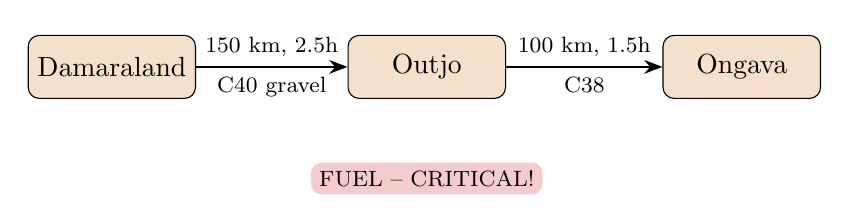
\begin{tikzpicture}[
    location/.style={rectangle, draw, fill=primarycolor!20, rounded corners, minimum width=2cm, minimum height=0.8cm},
    small/.style={font=\footnotesize}
]
\node[location] (start) at (0,0) {Damaraland};
\node[location] (outjo) at (4,0) {Outjo};
\node[location] (end) at (8,0) {Ongava};

\draw[->,>=Stealth,thick] (start) -- node[above,small] {150 km, 2.5h} node[below,small] {C40 gravel} (outjo);
\draw[->,>=Stealth,thick] (outjo) -- node[above,small] {100 km, 1.5h} node[below,small] {C38} (end);

\node[below=0.8cm of outjo, fill=warningcolor!20, rounded corners, inner sep=3pt, small] {FUEL -- CRITICAL!};
\end{tikzpicture}
\end{center}

\textbf{Timeline:}

\begin{tabular}{llr}
\toprule
\textbf{Time} & \textbf{Activity} & \textbf{Cost} \\
\midrule
08:00 & Depart Damaraland after breakfast & -- \\
10:30 & Fuel stop at Outjo (CRITICAL -- last station before Etosha) & €50 \\
14:00--15:00 & Arrive Ongava Lodge & -- \\
16:00 & First game drive into Etosha via private gate & Incl. \\
& Focus on Okaukuejo waterhole \& western plains & \\
After sunset & Transition to night drive on Ongava reserve & Incl. \\
Dinner & Overlooking floodlit waterhole; watch elephants while eating & Incl. \\
\bottomrule
\end{tabular}

\subsubsection{Day 11 (Jan 2): Western Etosha Exploration}

\begin{tabular}{llr}
\toprule
\textbf{Time} & \textbf{Activity} & \textbf{Cost} \\
\midrule
06:00--10:30 & Morning drive into Etosha & Incl. \\
& Explore Okaukuejo--Halali section & \\
& Check waterholes: Olifantsbad, Gemsbokvlakte & \\
& Scan pans for predators & \\
10:30 & Return to lodge; breakfast/brunch & -- \\
Midday & Pool \& waterhole watching from shaded deck & -- \\
16:00 & Afternoon drive on Ongava reserve & Incl. \\
& Sundowners at scenic viewpoint & \\
After sunset & Night drive spotting leopards/brown hyenas/aardwolf & Incl. \\
\bottomrule
\end{tabular}

\subsubsection{Day 12 (Jan 3): Transit to Eastern Etosha}

\textbf{Route:} Ongava (West) → Onguma (East) -- 200 km through park, 4--5 hours

\begin{tabular}{llr}
\toprule
\textbf{Time} & \textbf{Activity} & \textbf{Cost} \\
\midrule
06:00--13:00 & Morning drive \& transit through Etosha to eastern side & Incl. \\
& This internal park drive IS a game drive & \\
& Stop at multiple waterholes en route & \\
14:00 & Arrive Onguma The Fort; check-in & -- \\
& Explore fortress architecture \& tower & \\
16:00 & First drive into eastern Etosha via Von Lindequist Gate & Incl. \\
& Namutoni waterhole, Klein Namutoni (leopard hotspot) & \\
& Eastern grasslands (best for Jan green season) & \\
Sunset & View from Fort's tower overlooking Fischer's Pan & -- \\
After dark & Night drive on Onguma reserve & Incl. \\
\bottomrule
\end{tabular}

\clearpage
\subsubsection{Day 13 (Jan 4): Eastern Etosha -- Best January Viewing}

\begin{tabular}{llr}
\toprule
\textbf{Time} & \textbf{Activity} & \textbf{Cost} \\
\midrule
06:00--10:30 & Morning drive deep into eastern Etosha & Incl. \\
& \textit{Most productive sector during green season} & \\
& Focus on areas recommended by guides & \\
10:30 & Return to lodge & -- \\
Midday & Final waterhole watching, packing & -- \\
16:00 & Last evening drive on Onguma reserve & Incl. \\
Evening & Final night at The Fort & -- \\
\bottomrule
\end{tabular}

\subsubsection{Accommodation Options: Etosha (4 nights)}

\textbf{Status:} \tbdstatus

\textbf{Strategy:} Split 2 nights western + 2 nights eastern to maximize January success

\textbf{WESTERN ETOSHA (2 nights):}

\begin{enumerate}
    \item \textbf{Ongava Lodge} -- \textit{RECOMMENDED}
    \begin{itemize}
        \item 30,000-hectare private reserve bordering southern Etosha
        \item 14 rock-and-thatch chalets overlooking floodlit waterhole
        \item Active waterhole viewable 24/7 from restaurant/pool/rooms
        \item \textbf{Night drives in open 4x4s} (impossible in park)
        \item Private access gate to Etosha
        \item All inclusive: meals, drinks, 2x daily drives, night drives
        \item \textbf{Cost:} €1,650 for 2 nights (per person)
        \item \textbf{Pros:} Night drives, waterhole viewing, excellent guiding
        \item \textbf{Cons:} Expensive
    \end{itemize}

    \item \textbf{Ongava Tented Camp}
    \begin{itemize}
        \item Sister property, same reserve
        \item More intimate (8 tents)
        \item Same inclusions
        \item \textbf{Cost:} €1,500--1,700 for 2 nights (per person)
        \item \textbf{Pros:} Same benefits as Ongava Lodge, slightly less
        \item \textbf{Cons:} Still expensive
    \end{itemize}
\end{enumerate}

\textbf{EASTERN ETOSHA (2 nights):}

\begin{enumerate}
    \item \textbf{Onguma The Fort} -- \textit{RECOMMENDED}
    \begin{itemize}
        \item 35,970-hectare reserve bordering eastern Etosha
        \item North African kasbah-inspired fortress with tower
        \item 11 suites built around central tower
        \item Sunset views over Fischer's Pan
        \item Black rhino custodian zone (exceptional rhino sightings)
        \item Eastern sector = better for January/green season
        \item Night drives included
        \item Ethical viewing: max 3 vehicles per sighting
        \item \textbf{Cost:} €1,650 for 2 nights (per person)
        \item \textbf{Pros:} Best Jan location, night drives, unique architecture
        \item \textbf{Cons:} Expensive
    \end{itemize}

    \item \textbf{Onguma Tree Top Camp}
    \begin{itemize}
        \item Same reserve, 4 chalets elevated in trees
        \item Intimate, romantic
        \item \textbf{Cost:} €1,700--1,900 for 2 nights (per person)
        \item \textbf{Pros:} Unique treehouse experience
        \item \textbf{Cons:} Very small, likely booked
    \end{itemize}
\end{enumerate}

\clearpage
\textbf{BUDGET ALTERNATIVE (4 nights at one location):}

\begin{enumerate}
    \item \textbf{Mushara Lodge}
    \begin{itemize}
        \item 8 km from Von Lindequist Gate (eastern entrance)
        \item NOT on private concession (no night drives)
        \item Consistently praised for "best food in Namibia"
        \item Professional guides
        \item Eastern location good for January
        \item \textbf{Cost:} €1,600--2,000 for 4 nights (per person)
        \item \textbf{Pros:} Excellent value, outstanding food, good location, professional
        \item \textbf{Cons:} No night drives, no private waterhole
    \end{itemize}

    \item \textbf{Mokuti Etosha Lodge}
    \begin{itemize}
        \item Resort-style, 106 rooms (good availability)
        \item 4 waterholes on property for night viewing from hides
        \item Eastern gate access
        \item \textbf{Cost:} €1,400--1,800 for 4 nights (per person)
        \item \textbf{Pros:} Likely available, multiple waterholes, good facilities
        \item \textbf{Cons:} Large/impersonal, resort feel vs intimate safari
    \end{itemize}
\end{enumerate}

\subsubsection{January Green Season Reality Check}

\begin{itemize}
    \item \textbf{Challenge:} Summer rains create temporary pans everywhere; animals disperse
    \item \textbf{Advantage:} Springbok \& zebra calving attracts predators; green landscapes; dramatic thunderstorms
    \item \textbf{Strategy:} Eastern Etosha drains better = better game concentration in Jan--Apr
    \item \textbf{Private concessions:} Night drives \& expert guides change the equation
    \item \textbf{Expectation:} Work harder for sightings vs dry season's waterhole parades
\end{itemize}

\subsubsection{4-Day Budget Summary}

\begin{tabular}{@{}lr@{}}
\toprule
\textbf{Item} & \textbf{Cost (per person)} \\
\midrule
Accommodation (2n Ongava + 2n Onguma) & €3,300 \\
\textit{OR Mushara Lodge (4 nights)} & \textit{€1,800} \\
Fuel (250 km drive + park transit) & €70 \\
Park entry fees (3 days) & €25 \\
\midrule
\textbf{Total Days 10--13 (luxury)} & \textbf{€3,395} \\
\textbf{Total Days 10--13 (budget)} & \textbf{€1,895} \\
\bottomrule
\end{tabular}

\clearpage
% -----------------------------------------------------------------------------
\subsection{Day 14: January 5 -- Return to Windhoek}
% -----------------------------------------------------------------------------

\textbf{Route:} Etosha → Windhoek (430 km, 5--5.5 hours)

\begin{center}
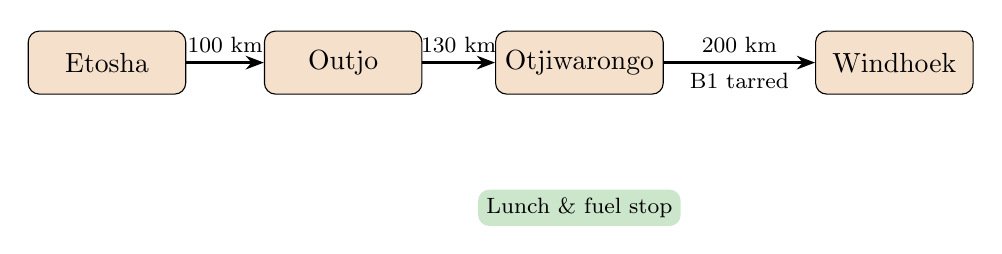
\begin{tikzpicture}[
    location/.style={rectangle, draw, fill=primarycolor!20, rounded corners, minimum width=2cm, minimum height=0.8cm},
    small/.style={font=\footnotesize}
]
\node[location] (start) at (0,0) {Etosha};
\node[location] (outjo) at (3,0) {Outjo};
\node[location] (otji) at (6,0) {Otjiwarongo};
\node[location] (end) at (10,0) {Windhoek};

\draw[->,>=Stealth,thick] (start) -- node[above,small] {100 km} (outjo);
\draw[->,>=Stealth,thick] (outjo) -- node[above,small] {130 km} (otji);
\draw[->,>=Stealth,thick] (otji) -- node[above,small] {200 km} node[below,small] {B1 tarred} (end);

\node[below=1.2cm of otji, fill=accentcolor!20, rounded corners, inner sep=3pt, small] {Lunch \& fuel stop};
\end{tikzpicture}
\end{center}

\textbf{Timeline:}

\begin{tabular}{llr}
\toprule
\textbf{Time} & \textbf{Activity} & \textbf{Cost} \\
\midrule
08:00 & Depart lodge after breakfast & -- \\
& Drive through park one final morning (game viewing as you transit) & -- \\
& Exit via Anderson Gate (if at Onguma, transit west through park) & -- \\
12:00 & Lunch stop at Otjiwarongo (coffee, fuel, bathroom) & €20 \\
& Optional: Okahandja craft market for souvenirs & €50 (opt) \\
15:00--16:00 & Arrive Windhoek & -- \\
& Return vehicle to rental company & -- \\
& Free shuttle to Airport Lodge & -- \\
Evening & Early dinner, pack, prepare for morning departure & €25 \\
\bottomrule
\end{tabular}

\subsubsection{Accommodation: Airport Lodge (Return)}

\textbf{Status:} \tbdstatus (Book for 1 night with free shuttle to airport)

\begin{itemize}
    \item Free shuttle to airport for morning departure
    \item Convenient location near airport
    \item Last-minute packing and preparation
\end{itemize}

\subsubsection{Vehicle Return Checklist}

\begin{itemize}
    \item Clean out all personal items
    \item Check for damage (document with photos if any)
    \item Fuel: Return with similar level as pickup (or pay refueling charge)
    \item Confirm final invoice \& insurance excess (if applicable)
    \item Get receipt and clear all charges
\end{itemize}

\subsubsection{Daily Budget}

\begin{tabular}{@{}lr@{}}
\toprule
\textbf{Item} & \textbf{Cost (per person)} \\
\midrule
Accommodation (Airport Lodge) & €65 \\
Fuel (430 km) & €60 \\
Meals & €45 \\
Souvenirs (optional) & €0--50 \\
\midrule
\textbf{Total Day 14} & \textbf{€170--220} \\
\bottomrule
\end{tabular}

\clearpage
% -----------------------------------------------------------------------------
\subsection{Day 15: January 6 -- Departure}
% -----------------------------------------------------------------------------

\begin{tabular}{llr}
\toprule
\textbf{Time} & \textbf{Activity} & \textbf{Cost} \\
\midrule
11:00 & Wake up, final packing & -- \\
12:00 & Shuttle to Hosea Kutako Airport (20 min) & Incl. \\
13:00 & Check-in for Ethiopian Airlines ET834 & -- \\
14:30 & \textbf{Depart Windhoek (WDH)} & -- \\
21:20 & Arrive Addis Ababa (ADD) -- 3h30 layover & -- \\
00:50 (Jan 7) & Depart ADD -- Ethiopian Airlines ET750 & -- \\
06:20 & \textbf{Arrive Brussels (BRU)} & -- \\
\bottomrule
\end{tabular}

\subsubsection{Pre-Departure Checklist}

\begin{itemize}
    \item Confirm flight time 24 hours prior
    \item Print boarding passes if possible
    \item Pack valuables in carry-on
    \item Keep passport, tickets, insurance docs accessible
    \item Check luggage weight limits
    \item Leave time for airport security
\end{itemize}

\clearpage
% =============================================================================
\section{Vehicle \& Driving Guide}
% =============================================================================

\subsection{Vehicle Rental: Toyota Hilux Double Cab 4x4}

\textbf{Status:} \tbdstatus

\textbf{Available Quote (Asco Car Hire):}
\begin{itemize}
    \item \textbf{Rental Company:} Asco Car Hire, Windhoek
    \item \textbf{Pick-up:} Dec 23, 2025, 15:30 -- Windhoek (Asco Car Hire Depot)
    \item \textbf{Return:} Jan 6, 2026, 14:30 -- Windhoek (Asco Car Hire Depot)
    \item \textbf{Duration:} 14 days (13 days 23 hours rental)
    \item \textbf{Cost:} €1,442 total (€288 per person) base rental
    \item \textbf{Insurance:} Add Option 3 coverage (+€360 est., €72 pp) for tire/windscreen
\end{itemize}

\textbf{Vehicle Specifications:}
\begin{itemize}
    \item \textbf{Model:} Toyota Hilux 2.4 Double Cab Automatic (2023-2025)
    \item Engine: 2.4L Diesel, Automatic Transmission
    \item 5 passengers, 5 doors, 4 large bags + 4 small bags
    \item Air Conditioning, Dual Battery System
    \item 4x4 with Rear Differential Lock
    \item 140L Fuel Tank, 40L Water Tank
    \item 2 Spare wheels, Unlimited mileage
    \item Power Steering, Airbags, ABS
    \item USB/AUX/Bluetooth, Central locking
    \item Offroad Tires, Electric windows
\end{itemize}

\textbf{Included Equipment:}
\begin{itemize}
    \item GPS navigation (Tracks4Africa recommended)
    \item High-lift jack and wheel tools
    \item Compressor for tire pressure adjustment
    \item First aid kit, fire extinguisher, warning triangle
    \item Black box for safety monitoring (tracks speed, location)
\end{itemize}

\subsection{Rental Companies}

\begin{enumerate}
    \item \textbf{Asco Car Hire}
    \begin{itemize}
        \item Email: info@ascocarhire.com
        \item Phone: +264 61 229 272
        \item Largest fleet, excellent maintenance, GPS tracking
    \end{itemize}

    \item \textbf{Advanced Car Hire}
    \begin{itemize}
        \item Email: info@advancedcarhire.com
        \item Phone: +264 81 287 6932
        \item Premium service, owner-managed, newer vehicles
    \end{itemize}
\end{enumerate}

\subsection{Insurance: CRITICAL}

\textbf{Get Option 3 or 4 coverage including:}
\begin{itemize}
    \item Tire damage (common on gravel)
    \item Windscreen damage (stone chips inevitable)
    \item Reduced excess from N\$40,000 ($\sim$€2,160) to manageable levels
    \item Cost: €360 total for 14 days (€72 per person)
    \item \textbf{This is the best money you'll spend}
\end{itemize}

\subsection{Gravel Road Driving Techniques}

\subsubsection{Speed Discipline}

\begin{itemize}
    \item GPS black box monitors speed
    \item \textcolor{warningcolor}{\textbf{Exceeding 80 km/h on gravel VOIDS ALL INSURANCE}}
    \item In accidents, data is analyzed -- if speeding, you pay full vehicle replacement ($\sim$€40,000)
    \item Comfortable cruising: 60 km/h on good gravel, 40--50 km/h on rough sections
    \item Corrugated "washboard" surfaces become uncontrollable above 70 km/h
\end{itemize}

\subsubsection{Corner Technique}

\begin{itemize}
    \item Gravel is slippery
    \item Slow to 40 km/h BEFORE curves
    \item Never brake mid-turn (causes fishtailing)
    \item Accelerate gently out of turn
    \item \textit{This single technique prevents 90\% of gravel road accidents}
\end{itemize}

\clearpage
\subsubsection{Tire Pressure Management}

\begin{itemize}
    \item Check at fuel stations
    \item Tarred roads: 2.4 bar
    \item Gravel roads: 1.8--2.0 bar (better traction \& comfort)
    \item Soft sand (last 7 km to Deadvlei): 1.5--1.8 bar
    \item Re-inflate when back on hard surfaces
\end{itemize}

\subsubsection{Oncoming Vehicles}

\begin{itemize}
    \item Approaching dust clouds obscure visibility completely
    \item Slow to 40 km/h, move far right
    \item Prepare to stop if necessary
    \item Never overtake in dust (can't see oncoming vehicles)
\end{itemize}

\subsubsection{Wildlife Encounters}

\begin{itemize}
    \item Animals on roads constant at dawn/dusk
    \item Oryx, kudus, warthogs, baboons cross unpredictably
    \item Drive 60 km/h maximum near parks and reserves
    \item \textcolor{warningcolor}{\textbf{NEVER drive after dark}} -- most accidents involve hitting animals at night
\end{itemize}

\subsection{Fuel Strategy}

\begin{itemize}
    \item \textbf{Fill up at EVERY opportunity}, even if only down to 3/4 tank
    \item Stations in remote areas sometimes run dry or have power outages
    \item Hilux has 145L capacity giving $\sim$900 km range
    \item Maintain 1/2 tank minimum always
    \item Pay cash (most stations don't accept cards)
\end{itemize}

\subsection{December-Specific Risks}

\begin{itemize}
    \item Summer rains create flash flooding
    \item If water crossing road: STOP, assess depth, watch other vehicles, proceed slowly in low gear
    \item If uncertain, wait for water to recede (1 hour patience beats getting stranded)
    \item Salt roads near coast extremely slippery in morning fog/mist -- reduce speed 50\%
\end{itemize}

\clearpage
% =============================================================================
\section{Accommodation Summary}
% =============================================================================

\begin{landscape}
\begin{longtable}{llllll}
\toprule
\textbf{Location} & \textbf{Property} & \textbf{Nights} & \textbf{Dates} & \textbf{Key Features} & \textbf{Cost/Person} \\
\midrule
\endfirsthead
\toprule
\textbf{Location} & \textbf{Property} & \textbf{Nights} & \textbf{Dates} & \textbf{Key Features} & \textbf{Cost/Person} \\
\midrule
\endhead
Windhoek & Airport Lodge & 1 & Jan 5 & Convenient, waterhole, free shuttle & €65 total \\
\midrule
Sossusvlei & Kulala Desert Lodge (LEADING) & 3 & Dec 24--26 & Private gate, all-inclusive, travel agent & €1,763 \\
& Sossusvlei Lodge (budget) & 3 & Dec 24--26 & At gate, functional, good value & €300--400 \\
\midrule
Swakopmund & Breeze Lodge (BOOKED) & 2 & Dec 27--28 & Swakopmund accommodation & TBD \\
\midrule
Damaraland & Damaraland Camp (1st) & 3 & Dec 29--31 & Best elephant tracking, community & €2,430 \\
& Mowani Mountain Camp (2nd) & 3 & Dec 29--31 & Luxury, boulders, A/C & €2,200--2,600 \\
\midrule
Etosha West & Ongava Lodge (recommended) & 2 & Jan 1--2 & Night drives, private waterhole & €1,650 \\
\midrule
Etosha East & Onguma The Fort (recommended) & 2 & Jan 3--4 & Best Jan sector, night drives & €1,650 \\
& Mushara Lodge (budget all 4n) & 4 & Jan 1--4 & Excellent food, professional, value & €1,600--2,000 \\
\bottomrule
\end{longtable}
\end{landscape}

\clearpage
% =============================================================================
\section{Budget Breakdown}
% =============================================================================

\subsection{Complete Cost Analysis}

\begin{longtable}{lrr}
\toprule
\textbf{Category} & \textbf{Per Person} & \textbf{Total (5 persons)} \\
\midrule
\endfirsthead
\toprule
\textbf{Category} & \textbf{Per Person} & \textbf{Total (5 persons)} \\
\midrule
\endhead
\multicolumn{3}{l}{\textbf{ACCOMMODATION (13 nights)}} \\
Airport Lodge (1n) & €65 & €325 \\
Sossusvlei -- Kulala Desert Lodge (3n) & €1,763 & €8,813 \\
Swakopmund -- The Stiltz (2n) & €80 & €400 \\
Damaraland Camp (3n) & €2,430 & €12,150 \\
Ongava Lodge (2n) & €1,650 & €8,250 \\
Onguma The Fort (2n) & €1,650 & €8,250 \\
\midrule
\textbf{Subtotal Accommodation} & \textbf{€7,638} & \textbf{€38,188} \\
\midrule
\multicolumn{3}{l}{\textbf{VEHICLE \& TRANSPORT}} \\
4x4 rental (14 days, Hilux) & €288 & €1,442 \\
Insurance upgrade (Option 3) & €72 & €360 \\
Fuel ($\sim$2,200 km, 8L/100km) & €365 & €1,825 \\
\midrule
\textbf{Subtotal Transport} & \textbf{€725} & \textbf{€3,627} \\
\midrule
\multicolumn{3}{l}{\textbf{ACTIVITIES}} \\
Hot air balloon (Sossusvlei) & €496 & €2,480 \\
Sandwich Harbour 4x4 & €145 & €725 \\
Cape Cross entry & €10 & €50 \\
Optional Twyfelfontein & €0--60 & €0--300 \\
\midrule
\textbf{Subtotal Activities} & \textbf{€651--711} & \textbf{€3,255--3,555} \\
\midrule
\multicolumn{3}{l}{\textbf{PARK FEES}} \\
Etosha entry (3 days) & €25 & €125 \\
Namib-Naukluft (Sossusvlei) & €25 & €125 \\
Vehicle fees & €10 & €50 \\
\midrule
\textbf{Subtotal Park Fees} & \textbf{€60} & \textbf{€300} \\
\midrule
\multicolumn{3}{l}{\textbf{MEALS (not included)}} \\
Swakopmund meals & €55 & €275 \\
Windhoek/Otjiwarongo stops & €95 & €475 \\
Snacks \& drinks & €50 & €250 \\
\midrule
\textbf{Subtotal Meals} & \textbf{€200} & \textbf{€1,000} \\
\midrule
\midrule
\textbf{GRAND TOTAL (excl. flights)} & \textbf{€9,214--9,274} & \textbf{€46,070--46,370} \\
\bottomrule
\end{longtable}

\subsection{Budget vs Target}

\begin{itemize}
    \item \textbf{Target budget:} €7,000 per person
    \item \textbf{Current budget (luxury):} €9,214--9,274 per person
    \item \textbf{Status:} \textcolor{warningcolor}{€2,214--2,274 over budget}
    \item \textbf{Solution:} Use Mushara Lodge for Etosha (saves €1,500 pp) to reach €7,714--7,774 per person
    \item \textbf{Note:} Kulala Desert Lodge all-inclusive pricing (€1,763 pp) includes meals \& activities that would cost extra elsewhere
\end{itemize}

\subsection{Cost-Saving Options to Meet Budget}

To meet the €7,000 per person target:

\begin{enumerate}
    \item \textbf{Replace Ongava/Onguma with Mushara Lodge} (4 nights): Save €1,500 per person
    \item With this change: €7,000--7,260 per person (within budget)
    \item Alternative: Use Sossusvlei Lodge instead of Kulala: Save €400 per person
    \item Skip hot air balloon: Save €540 per person (NOT RECOMMENDED)
\end{enumerate}

\clearpage
% =============================================================================
\section{Packing List}
% =============================================================================

\subsection{Clothing (Neutral Colors: Khaki, Olive, Tan)}

\textbf{Temperature Range:} 15--40°C daily swings require layering

\begin{itemize}
    \item Convertible zip-off pants (3 pairs) -- zip off to shorts by 10am
    \item Long-sleeve lightweight shirts (3) -- sun protection, breathable
    \item Short-sleeve shirts (3)
    \item Fleece or hoodie -- \textbf{ESSENTIAL} for 5:30am game drives
    \item Light rain jacket (packable, waterproof) -- afternoon thunderstorms
    \item Wide-brim sun hat -- non-negotiable in desert
    \item Warm hat/beanie for early morning drives
    \item Closed walking shoes (trail runners perfect; hiking boots overkill)
    \item Sandals for lodge use
    \item Swimsuit -- essential for cooling off in 40°C heat
    \item Buff or light scarf -- dust protection on gravel roads
\end{itemize}

\subsection{Electronics}

\begin{itemize}
    \item Camera with telephoto zoom (200--400mm ideal for wildlife)
    \item Binoculars -- \textbf{ABSOLUTELY ESSENTIAL} (5 pairs needed!)
    \item Power bank (10,000+ mAh)
    \item Headlamp with red light setting
    \item Travel adapter (Type D \& M plugs -- South African 3 large round pins)
    \item Car charger with dual USB ports
    \item Memory cards (extra for all photos)
\end{itemize}

\subsection{Sun Protection (Buy in Belgium -- Expensive in Namibia)}

\begin{itemize}
    \item Sunscreen SPF 50+ (200ml minimum per person, reapply constantly)
    \item Lip balm with SPF
    \item Sunglasses (polarized for glare) -- 5 pairs
    \item After-sun lotion
\end{itemize}

\subsection{Practical Items}

\begin{itemize}
    \item Reusable water bottles (1L per person minimum)
    \item Day backpack for game drives
    \item Ziplock bags -- dust-proof electronics when driving gravel
    \item Small first aid kit (plasters, antiseptic, paracetamol, anti-diarrheal)
    \item Insect repellent (buy locally in Windhoek -- DEET 50\%)
    \item Wet wipes/hand sanitizer
    \item Tissues/toilet paper (emergency roadside situations)
\end{itemize}

\subsection{Documents}

\begin{itemize}
    \item Passports (valid 6+ months beyond Jan 6, minimum 2 empty visa pages) -- 5 passports
    \item Driver's licenses (all who will drive)
    \item International Driving Permit (recommended but not legally required)
    \item Travel insurance policy with emergency numbers
    \item Accommodation confirmations (printed \& digital)
    \item Vehicle rental voucher
    \item Credit cards (Visa/Mastercard) + ATM cards
    \item Emergency cash: €200--300 equivalent
\end{itemize}

\subsection{What NOT to Pack}

\begin{itemize}
    \item Heavy jeans (too hot, too heavy)
    \item Formal wear (lodges are safari-casual)
    \item Dark colors (attract heat and tsetse flies)
    \item Bright white (shows every dust particle after first gravel road)
    \item Hard-shell luggage (won't fit in some vehicles, difficult to store)
\end{itemize}

\clearpage
% =============================================================================
\section{Safety \& Practical Information}
% =============================================================================

\subsection{Wildlife Safety (Critical)}

\begin{itemize}
    \item \textcolor{warningcolor}{\textbf{Stay in vehicle always}} in national parks
    \item Stepping out = death sentence if lion/elephant nearby
    \item Windows closed when near predators or elephants
    \item Never approach elephants on foot (tracking done WITH professional guides)
    \item Baboons at rest stops steal food through open windows in seconds
    \item Don't feed or approach any animals
    \item At lodge waterholes, observe from designated viewing areas only
\end{itemize}

\subsection{Medical Preparation}

\begin{itemize}
    \item Namibia is malaria-free except far northern regions (not visiting)
    \item No required vaccinations
    \item Travel insurance with medical evacuation ESSENTIAL (5 people coverage)
    \item Private healthcare in Windhoek/Swakopmund good; rural areas have clinics only
    \item Carry comprehensive first aid kit
    \item Prescription medications: Bring 150\% of what you need
\end{itemize}

\subsection{Communications \& Emergency}

\begin{itemize}
    \item Cell coverage good in towns, limited in parks and desert
    \item Buy MTC SIM card at Windhoek airport (N\$50--100 with airtime)
    \item Emergency numbers: 10111 (police), +264 81 241 7555 (ER24)
    \item Lodges have satellite phones or radios for emergencies
    \item Inform lodges of your route when departing
    \item Tell family your itinerary before entering remote areas
\end{itemize}

\subsection{Water Safety}

\begin{itemize}
    \item Tap water in cities: Safe to drink
    \item Lodges: Usually filtered/treated, ask staff
    \item Remote areas: Bottled water only
    \item Dehydration danger in desert: Drink 4--5L daily even if not thirsty
    \item Signs of dehydration: Headache, dizziness, dark urine -- rest in shade, drink immediately
\end{itemize}

\subsection{Weather Hazards}

\begin{itemize}
    \item Heat exhaustion/heat stroke in Sossusvlei: Stay shaded 11am--4pm
    \item Wear hat, drink constantly, recognize symptoms (confusion, nausea, rapid heartbeat)
    \item Thunderstorms: Spectacular but can include flash flooding
    \item If water crossing road, wait for level to drop
    \item Lightning common in January -- seek vehicle or building immediately if caught outside
    \item Sun exposure: Reapply sunscreen every 2 hours; desert sun at altitude is brutal
\end{itemize}

\clearpage
% =============================================================================
\section{Booking Action Plan}
% =============================================================================

\subsection{CRITICAL: Act Within 48 Hours}

Six weeks before Christmas is catastrophically late for Christmas/New Year bookings in Namibia. Properties book 8--12 months ahead for festive season.

\subsection{Immediate Actions (Today/Tomorrow)}

\subsubsection{1. Contact Tour Operator (Recommended Approach)}

Use established operators rather than booking direct:

\begin{itemize}
    \item \textbf{Expert Africa:} www.expertafrica.com | +44 203 405 6666
    \item \textbf{Yellow Zebra Safaris:} www.yellowzebrasafaris.com
    \item \textbf{Wilderness Safaris:} www.wildernessdestinations.com (for Kulala/Damaraland/Ongava)
\end{itemize}

\textbf{Tell them:}
\begin{quote}
``We need December 23--January 6, Belgian family of 5, priority on wildlife access, €7,000 per person budget. What's actually available?''
\end{quote}

\textbf{Tour operators have:}
\begin{itemize}
    \item Allocation/blocked rooms at lodges
    \item Relationships allowing access to ``fully booked'' properties
    \item Real-time availability knowledge
    \item Emergency contacts for last-minute changes
    \item Single invoice consolidating everything
\end{itemize}

\subsubsection{2. Book Activities Independently (NOW)}

\begin{enumerate}
    \item \textbf{Hot Air Balloon:}
    \begin{itemize}
        \item Company: Namib Sky Balloon Safaris
        \item Website: www.balloon-safaris.com
        \item Phone: +264 63 293 233
        \item Date needed: December 26 (closed Dec 25 \& Jan 1)
    \end{itemize}

    \item \textbf{Sandwich Harbour 4x4:}
    \begin{itemize}
        \item Company: Sandwich Harbour 4x4
        \item Website: www.sandwich-harbour.com
        \item Phone: +264 81 128 6388
        \item Date needed: December 28
    \end{itemize}
\end{enumerate}

\subsubsection{3. Reserve Vehicle}

Contact immediately:

\begin{itemize}
    \item \textbf{Asco Car Hire:} info@ascocarhire.com | +264 61 229 272
    \item \textbf{Advanced Car Hire:} info@advancedcarhire.com | +264 81 287 6932
\end{itemize}

\textbf{Specify:}
\begin{itemize}
    \item Toyota Hilux Double Cab 4x4
    \item Automatic transmission (if preferred)
    \item December 24 (afternoon) pickup, January 5 (afternoon) return
    \item Option 3 or 4 insurance with tire/windscreen coverage
    \item Confirm: GPS with Tracks4Africa, dual spare tires, compressor, free airport shuttle
\end{itemize}

\subsection{Payment Terms}

\begin{itemize}
    \item Expect to pay 100\% upfront (normal is 50\% deposit, but you're inside 60-day window)
    \item Most lodges accept Visa/Mastercard
    \item Request billing in EUR to avoid exchange rate uncertainty
    \item Cancellation policies during festive season are strict (60--90 days notice, many non-refundable)
    \item \textbf{Purchase comprehensive travel insurance immediately for 5 people}
\end{itemize}

\subsection{Availability Reality Check}

\textbf{If properties fully booked, accept alternatives:}

\begin{itemize}
    \item Little Kulala → Kulala Desert Lodge (same private access)
    \item Kulala → Sossusvlei Lodge (functional, good value)
    \item Damaraland Camp → Mowani Mountain Camp (good elephant success)
    \item Ongava/Onguma → Mushara Lodge (excellent value, no night drives but professional)
\end{itemize}

\clearpage
% =============================================================================
\section{Contact Directory}
% =============================================================================

\subsection{Tour Operators}

\begin{tabular}{@{}lll@{}}
\toprule
\textbf{Company} & \textbf{Contact} & \textbf{Notes} \\
\midrule
Expert Africa & +44 203 405 6666 & www.expertafrica.com \\
& & Comprehensive Namibia specialists \\
Yellow Zebra Safaris & -- & www.yellowzebrasafaris.com \\
& & Southern Africa focus \\
Wilderness Safaris & -- & www.wildernessdestinations.com \\
& & Direct for Wilderness properties \\
\bottomrule
\end{tabular}

\subsection{Activities}

\begin{tabular}{@{}lll@{}}
\toprule
\textbf{Activity} & \textbf{Contact} & \textbf{Notes} \\
\midrule
Namib Sky Balloon Safaris & +264 63 293 233 & www.balloon-safaris.com \\
& & Book Dec 26 slot (5 people) \\
Sandwich Harbour 4x4 & +264 81 128 6388 & www.sandwich-harbour.com \\
& & Book Dec 28 tour (5 people) \\
\bottomrule
\end{tabular}

\subsection{Vehicle Rental}

\begin{tabular}{@{}lll@{}}
\toprule
\textbf{Company} & \textbf{Contact} & \textbf{Email} \\
\midrule
Asco Car Hire & +264 61 229 272 & info@ascocarhire.com \\
Advanced Car Hire & +264 81 287 6932 & info@advancedcarhire.com \\
\bottomrule
\end{tabular}

\subsection{Accommodations (Direct Booking if Needed)}

\begin{tabular}{@{}ll@{}}
\toprule
\textbf{Property} & \textbf{Contact} \\
\midrule
Airport Lodge & www.airportlodge.com.na \\
Wilderness Little Kulala & reservations@wilderness.co.za \\
Wilderness Kulala Desert Lodge & reservations@wilderness.co.za \\
The Stiltz & www.thestiltz.com \\
Wilderness Damaraland Camp & reservations@wilderness.co.za \\
Mowani Mountain Camp & www.mowani.com \\
Ongava Lodge & reservations@ongava.com \\
Onguma The Fort & reservations@onguma.com \\
Mushara Lodge & www.mushara-lodge.com \\
\bottomrule
\end{tabular}

\subsection{Emergency Services}

\begin{tabular}{@{}ll@{}}
\toprule
\textbf{Service} & \textbf{Number} \\
\midrule
Police Emergency & 10111 \\
ER24 Private Emergency & +264 81 241 7555 \\
Fire & 211111 \\
Ambulance & 211111 \\
Car Rental Emergency & [From rental company] \\
Travel Insurance Emergency & [Your policy number] \\
\bottomrule
\end{tabular}

\clearpage
% =============================================================================
\section{Notes \& Updates}
% =============================================================================

\subsection{Booking Status Tracker}

\textit{Update this section as bookings are confirmed:}

\vspace{1em}
\begin{tabular}{lll}
\toprule
\textbf{Item} & \textbf{Status} & \textbf{Confirmation \#} \\
\midrule
Airport Lodge & \tbdstatus & \\
Sossusvlei accommodation (Kulala) & \option & Via travel agent \\
Breeze Lodge, Swakopmund & \booked & TBD \\
Damaraland accommodation & \tbdstatus & \\
Etosha West accommodation & \tbdstatus & \\
Etosha East accommodation & \tbdstatus & \\
\midrule
Hot air balloon (Dec 26) - 5 people & \option & 2201704 (pending payment) \\
Sandwich Harbour 4x4 (Dec 28) - 5 people & \tbdstatus & \\
\midrule
Vehicle rental (Dec 24--Jan 5) & \tbdstatus & \\
Travel insurance (5 people) & \tbdstatus & \\
\midrule
International flights & \tbdstatus & \\
\bottomrule
\end{tabular}

\subsection{Changes \& Modifications}

\textit{Document any changes to the itinerary here:}

\vspace{3em}

\subsection{Additional Notes}

\vspace{5em}

% =============================================================================
% End of Document
% =============================================================================

\end{document}
